% =========================================================================
\chapter{Results and what they mean}
\label{ch:results}
% =========================================================================

\section{Main result: severe days}
\begin{center}
\begin{tabular}{lccc}
\toprule
\textbf{Training data} & \textbf{Severe PR-AUC} & \textbf{Change} & \textbf{All days}\\
\midrule
Real data only & 0.441 & -- & 0.599\\
Real + DDPM & 0.579 & +31\% & 0.609--0.611\\
Real + TVAE & 0.601 & +36\% & 0.609--0.611\\
Real + CTGAN & 0.601 & +36\% & 0.609--0.611\\
\bottomrule
\end{tabular}
\end{center}
Combined (5-seed ensemble) scores. Adding EVT-guided synthetic extremes raises the severe score by about a third, while
the all-days score also rises slightly, so nothing is lost on ordinary extremes.

\begin{figure}[H]
\centering
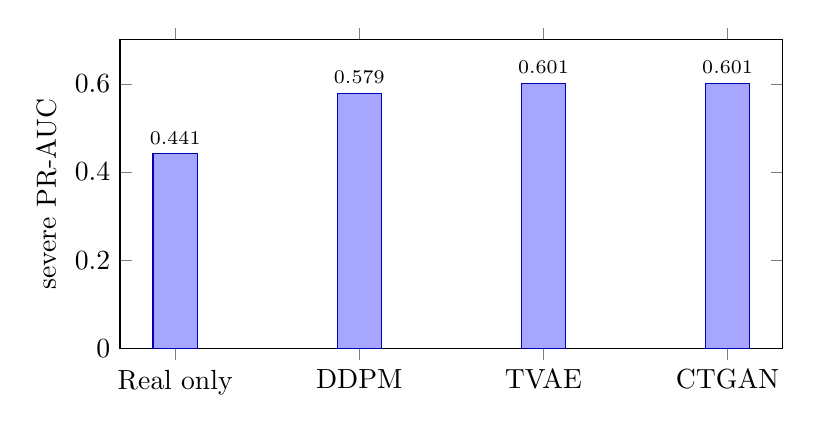
\begin{tikzpicture}
\begin{axis}[ybar,width=10cm,height=5.5cm,bar width=16pt,ymin=0,ymax=0.7,ylabel={severe PR-AUC},
  symbolic x coords={Real only,DDPM,TVAE,CTGAN},xtick=data,nodes near coords,
  nodes near coords style={font=\scriptsize},every node near coord/.append style={/pgf/number format/fixed,/pgf/number format/precision=3}]
\addplot[fill=blue!35,draw=blue!70!black] coordinates {(Real only,0.441)(DDPM,0.579)(TVAE,0.601)(CTGAN,0.601)};
\end{axis}
\end{tikzpicture}
\caption{Severe-day PR-AUC, combined model.}
\end{figure}

\section{Does the EVT tail matter? (per-seed means, severe days)}
\begin{center}
\begin{tabular}{lcccc}
\toprule
\textbf{Generator} & \textbf{Plain} & \textbf{EVT tail} & \textbf{Gain} & \textbf{Runs better}\\
\midrule
DDPM & 0.482 & 0.549 & +13.8\% & 5/5\\
TVAE & 0.514 & 0.583 & +13.6\% & 5/5\\
CTGAN & 0.554 & 0.581 & +4.9\% & 3/5\\
\bottomrule
\end{tabular}
\end{center}
``Plain'' = the same number of synthetic days, but chosen without EVT (their severities follow the generator).
Real data only scores 0.411 on this per-seed basis. EVT helps all three; it helps CTGAN least because CTGAN already
reaches the hot tail by itself.

\section{Checks that support the method}
\begin{itemize}
  \item \textbf{GPD as-is} (sample tail positions straight from the fitted GPD, no extra weight on the top fifth):
        0.462, better in only 1 of 5 runs. The \emph{tail focus} is what helps.
  \item \textbf{Random copies control:} adding copies of random real extremes gives 0.464; copying real extremes
        chosen by the EVT tail rule gives 0.521 (5/5, all-days 0.608). So the tail rule helps even without a
        generator, and new generated days help more.
  \item \textbf{How many to add:} 1 synthetic per real extreme gave onset 0.222; 8.7 per extreme gave 0.197. More is not
        better: too many synthetic days drown the real ones.
\end{itemize}

\section{In practice (CTGAN, combined model, chosen cut-off)}
Precision 0.600, recall 0.550, false-alarm rate 0.7\%: of every 10 warnings, 6 are right; a little over half of the
extreme days are warned; fewer than 1 in 100 normal days gets a false warning.

\section{Limitations (say these before they are asked)}
\begin{itemize}
  \item One region and one dataset (ERA5-Land, a reanalysis, not station readings; not bias-corrected).
  \item Thresholds come from 1981--2010; the test years are warmer (1.94\% extremes vs 1\%), so the task shifts.
  \item Synthetic days are judged only by whether they help the classifier, not checked by a meteorologist.
  \item GPD fitted by pooling cells within a season; it ignores differences between cells.
  \item Only next-day prediction; longer lead times were not tried.
\end{itemize}

\begin{sayit}
``With real data alone the severe score is 0.441. Adding EVT-guided synthetic extremes raises it to 0.58--0.60, about
a third better, without hurting the all-days score. The controls show the gain comes from focusing on the tail, not
just from adding more rows.''
\end{sayit}
